\section{The Identity-Transformation Approach}
\label{sec:challenge}

We discuss the security requirements of privacy-preserving SSO and present the identity-transformation approach.


\subsection{Security Requirements of for SSO Services}
\label{subsec:basicrequirements}

Non-anonymous SSO Services \cite{OpenIDConnect,rfc6749,SAML,SAMLIdentifier,NIST2017draft} are designed to allow a \emph{legitimate} user to login to an \emph{honest} RP with her permanent account at that RP, %correlating multiple login instances,
by presenting \emph{identity tokens} issued by a \emph{trusted} IdP. To achieve this goal, the trusted IdP issues an identity token that specifies the RP being accessed (i.e., \emph{RP designation}) and  the authenticated user's identity (i.e., \emph{user identification}). An honest RP verifies the requested RP's identity (or pseudo-identity) in the identity token before accepting it and authorizes the token holder to login as the specified user. This prevents malicious RPs from replaying received identity tokens to gain unauthorized access to other honest RPs as the victim user.
\emph{Confidentiality} and \emph{integrity} of identity tokens are also critical to prevent eavesdropping and tampering in SSO. Identity tokens must be forwarded to the target RPs by the authenticated user and should not be revealed to any other parties. %Otherwise, an eavesdropper who possesses the token could successfully login to the designated RP. Maintaining integrity is also critical to prevent adversaries from tampering with a token. So,
They are usually signed by the trusted IdP and transmitted over HTTPS \cite{OpenIDConnect,rfc6749,SAML}.

The requirements for secure SSO services, i.e., {\bf {\em RP designation, user identification,}} and the {\bf {\em integrity and confidentiality of identity tokens}}, have been extensively studied in the literature \cite{ArmandoCCCT08, FettKS16, FettKS17}.
Any vulnerabilities that undermine these properties result in various attacks \cite{SomorovskyMSKJ12, WangCW12, ArmandoCCCPS13, ZhouE14, WangZLLYLG15, WangZLG16, YangLLZH16, MainkaMS16, MainkaMSW17, YangLCZ18, YangLS17, ShiWL19, ChenPCTKT14, ccsSunB12, DiscoveringJCS, dimvaLiM16, CaoSBKVC14, TowardsShehabM14}.


%\subsection{The Identity Dilemma of Privacy-Preserving SSO}
%\label{subsec:challenges}
\begin{table}
\footnotesize
    \caption{The (pseudo-)identities in privacy-preserving SSO}
    \centering
%    \begin{tabular}{|l|l|l|}
    \begin{tabular}{|p{1.0cm}|p{5.1cm}|p{1.13cm}|} \hline
    {\textbf{Notation}} & {\textbf{Description}} & {\textbf{Lifecycle}} \\ \hline
    {$ID_U$} & {The user's unique identity at the IdP.} & {Permanent} \\ \hline
    {$ID_{RP_j}$} & {The $j$-th RP's unique identity at the IdP.} & {Permanent} \\ \hline
    {$PID_{U,j}^i$} & {The user's pseudo-identity in her $i$-th login instance to the $j$-th RP.} & {Ephemeral} \\ \hline
    {$PID_{RP_j}^i$} & {The $j$-th RP's pseudo-identity in the user's $i$-th login instance to that RP.} & {Ephemeral} \\ \hline
    {$Acct_j$} & {The user's identity (or account) at the $j$-th RP.} & {Permanent} \\ \hline
    \end{tabular}
    \label{tbl:notations-dilemma}
\end{table}

\subsection{Identity Transformation}
\label{subsec:solutions}

\textcolor{blue}{We aim to develop a privacy-preserving SSO system that ensures the four security properties while preventing both IdP-based login tracing and RP-based identity linkage.
%We explicitly distinguish a user's identity (or \emph{account}) at an RP,
%     from the user's \emph{identity} at an IdP and the user's \emph{pseudo-identities} enclosed in identity tokens.
In UPPRESSO, these requirements are satisfied through \emph{transformed identities} in the identity tokens. Table \ref{tbl:notations-dilemma} lists the notations used in this paper.
The subscript $j$ and/or the superscript $i$ may be ignored if it does not cause ambiguity.}

\textcolor{blue}{In an SSO login flow,
a user initiates the process by negotiating an \emph{ephemeral} pseudonymous identity $PID_{RP}$  with the target RP and sending an identity token request that includes $PID_{RP}$ to the IdP.
Upon successful authentication of the user as $ID_U$, the IdP calculates an \emph{ephemeral} $PID_U$ based on $ID_U$ and $PID_{RP}$ and issues an identity token that binds $PID_U$ and $PID_{RP}$. Upon receiving a token with a matching $PID_{RP}$, the RP calculates the user's \emph{permanent} $Acct$ and authorizes the token holder to login.
%
%Given a user,
%    (\emph{a}) an identity token contains only pseudo-identities, i.e., $PID_{U,j}^i$ and $PID_{RP_j}^i$,
%        which are independent of each other for different RPs and in multiple login instances, respectively,
%    and (\emph{b}) these \emph{ephemeral} pseudo-identities enable the target RP to derive a \emph{permanent} account, i.e., $Acct_j$.
The relationships among the permanent and ephemeral (pseudo-)identities are depicted in Figure \ref{fig:IDCorrelation}, where the \emph{red} and \emph{green} blocks represent \emph{permanent} and \emph{ephemeral} (pseudo-)identities, respectively, and
the labeled arrows denote the transformations of (pseudo-)identities.}
%It describes the {\em identity dilemma} of privacy-preserving SSO as below:

%An identity token binds the (pseudo-)identities of an authenticated user and an RP.
%Since an IdP authenticates users and then always knows the user's identity (i.e., $ID_U$),
%    to prevent the IdP-based login tracing,
%    we should not reveal the target RP's permanent identity (i.e., $ID_{RP}$) to the IdP.

\textcolor{blue}{To guarantee RP designation, $PID_{RP}$ should be \emph{uniquely} associated with the target RP.
For user identification, the \emph{ephemeral} $PID_{U}^i$ in each login instance should enable the RP to derive the user's \emph{permanent} account  ($Acct$) at that RP.
To prevent IdP-based login tracing, it is essential to ensure that the IdP does not obtain any information about $ID_{RP}$ from any $PID_{RP}^i$. Therefore, in a user's multiple login instances to the same RP, he should generate independent $PID_{RP}^i$\footnote{The IdP should not be able to link multiple login instances to a given RP, even when the RP's identity is unknown to the IdP.} % the IdP-based login tracing is still effective, to correlate a user's multiple login instances.
and independent $PID_U^i$\footnote{If $PID_U^i$ is not completely independent of each other, it implies that there is a possibility for the IdP to link multiple login instances to a given RP.}.
Finally, to prevent RP-based identity linkage,
% the IdP does not enclose $ID_U$ in identity tokens.
%a user pseudo-identity (i.e., $PID_U$) is bound instead:
%$PID_U$ is bound in identity tokens:
the RP should not obtain any information about $ID_U$ from any $PID_{U,j}$, which implies that $PID_{U,j}$ for different RPs should also be independent of each other.
Therefore, we propose three identity transformations as follows:
\vspace{-\topsep}\begin{itemize}
\setlength{\topsep}{0pt}
\setlength{\partopsep}{0pt}
\setlength{\itemsep}{0pt}
\setlength{\parsep}{0pt}
\setlength{\parskip}{0pt}
\item
$\mathcal{F}_{PID_{RP}}(ID_{RP}) = PID_{RP}$, calculated by the user and the RP.
From the IdP's view,
$\mathcal{F}_{PID_{RP}}()$ is a one-way function and $PID_{RP}$
is \emph{indistinguishable} from random variables.
\item
$\mathcal{F}_{PID_U}(ID_U, PID_{RP}) = PID_{U}$, calculated by the IdP.
From the target RP's view,
    $\mathcal{F}_{PID_U}()$ is a one-way function and $PID_{U}$ is \emph{indistinguishable} from random variables.
\item
$\mathcal{F}_{Acct}(PID_{U}, PID_{RP}) = Acct$, calculated by the RP.
Given $ID_U$ and $ID_{RP}$, $Acct$ is %\emph{permanent} and
\emph{unique} to other accounts at that RP.
In a user's any two different login instances to the RP,
 $\mathcal{F}_{Acct}(PID_{U}^i, PID_{RP}^i) = \mathcal{F}_{Acct}(PID_{U}^{i'}, PID_{RP}^{i'})$.
\end{itemize}}

\begin{figure}[bt]
  \centering
  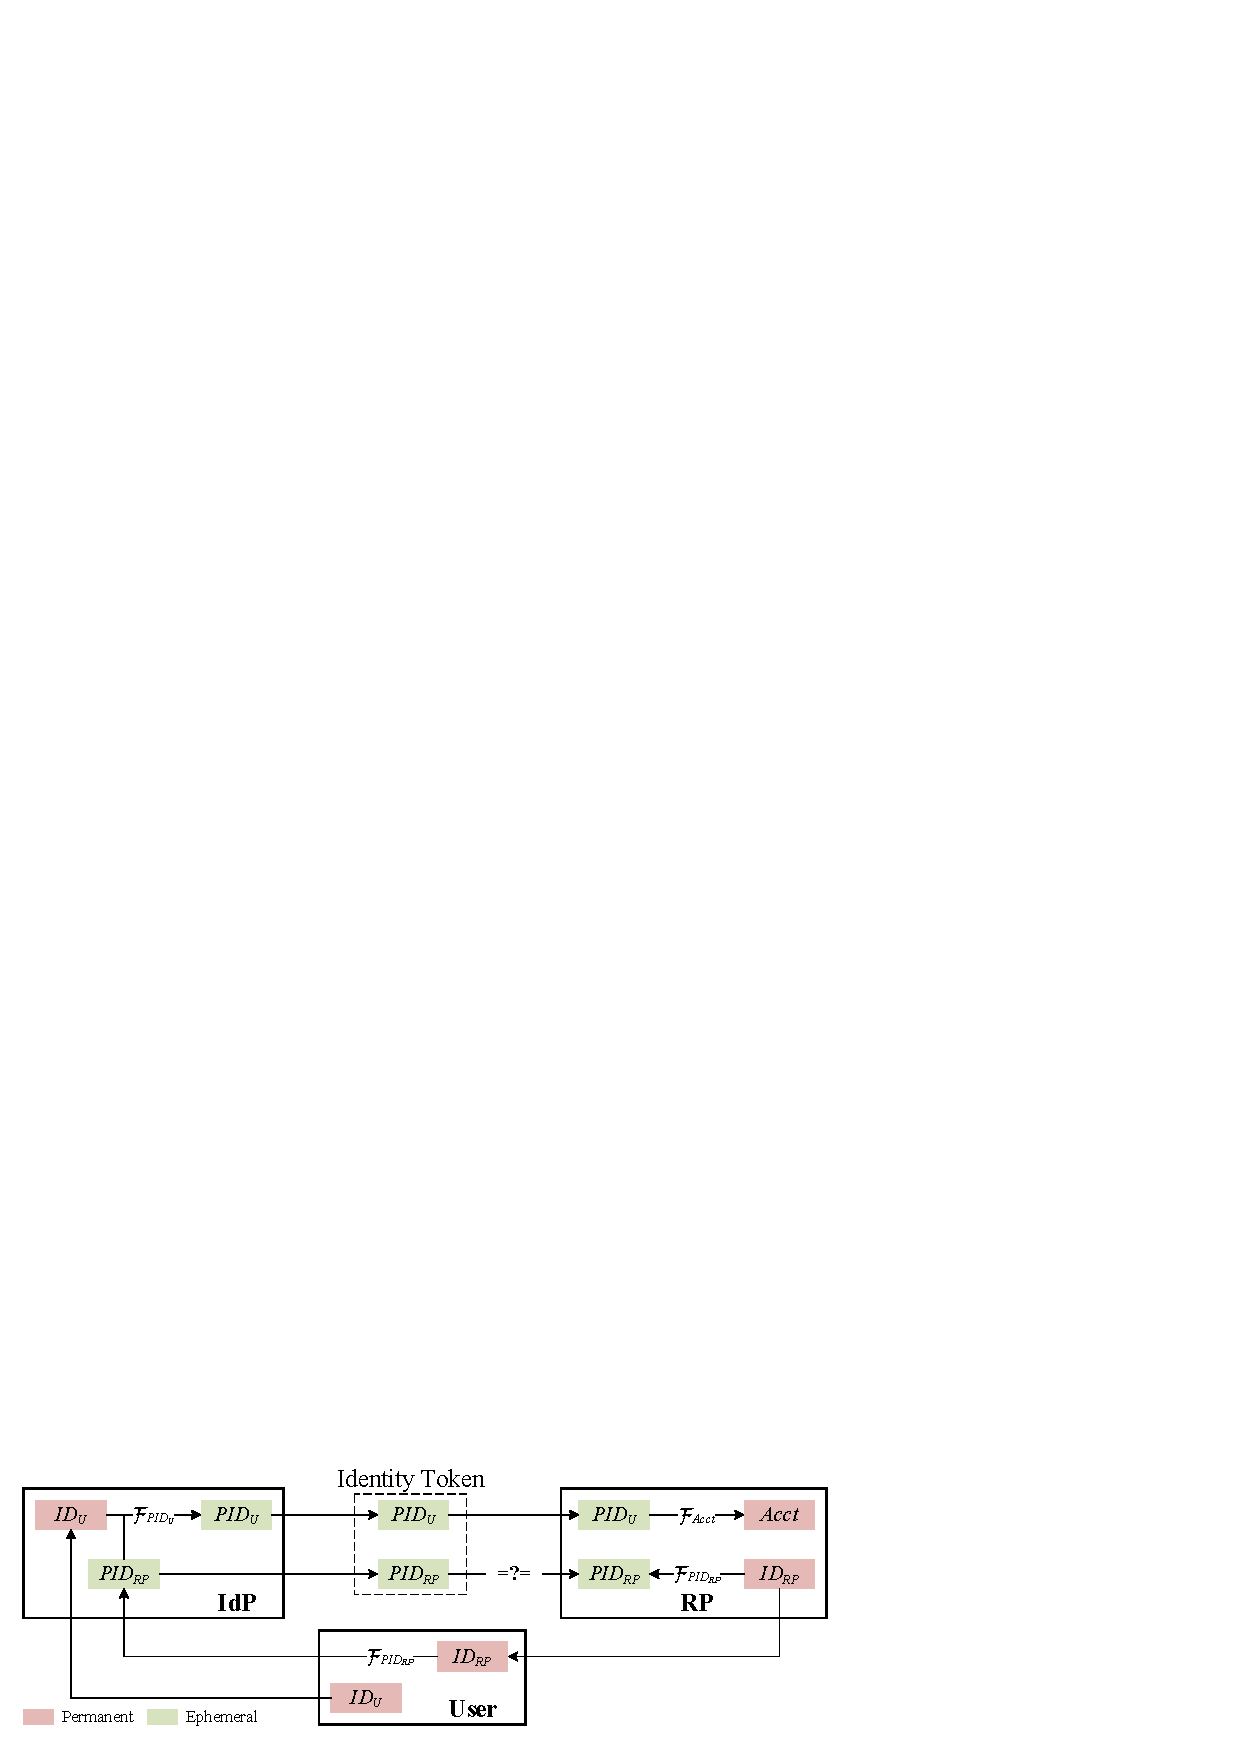
\includegraphics[width=0.99\linewidth]{fig/IDCorrelation.pdf}
  \caption{Identity transformations in privacy-preserving SSO}
  \label{fig:IDCorrelation}
\end{figure}

%We pose the \emph{identity dilemma} (or challenge) of SSO identity tokens
%    to satisfy the requirements of both security and privacy:
%
%\noindent\emph{Given an authenticated user and an unknown RP (i.e., permanent $ID_U$ and ephemeral $PID_{RP}$),
%    an IdP is expected to generate an ephemeral pseudo-identity (i.e., $PID_{U}$)
%     which will be correlated with the user's permanent identity at this RP (i.e., $Acct$),
%     while knowing nothing about the RP's identity or the user's account at this RP (i.e., $ID_{RP}$ or $Acct$).}

%Existing privacy-preserving SSO solutions (i.e., SPRESSO \cite{SPRESSO}, BrowserID \cite{BrowserID} and PPID \cite{NIST2017draft})
%  do not explicitly and comprehensively consider all five (pseudo-)identities in the SSO login flow,
%    and $ID_U$ or $ID_{RP}$ is still enclosed in identity tokens.
%So only one type of privacy threat is prevented.



